% Generated from reviewed lane; compile via book/textbook.tex.
\clearpage

原书 PDF 页 233；印刷页码 220。

\href{source-images/pdf-233.jpeg}{原页图像}

\section{第 9 章 矩阵的特征值与特征向量计算}\label{ch09a-ux7b2c-9-ux7ae0-ux77e9ux9635ux7684ux7279ux5f81ux503cux4e0eux7279ux5f81ux5411ux91cfux8ba1ux7b97}

\subsection{9.1 引言}\label{ch09a-ux5f15ux8a00}

物理、力学和工程技术中的很多问题在数学上都归结为求矩阵特征值的问题，例如振动问题（桥梁的振动、机械的振动、电磁振荡、地震引起的建筑物的振动等）、物理学中某些临界值的确定问题以及理论物理中的一些问题。这些实际问题可归结为如下数学问题。

（1）已知 \(A=(a_{ij})_{n\times n}\)，要求代数方程

\[
\varphi(\lambda)=\det(\lambda I-A)=0
\tag{9.1.1}
\]

的根。\(\varphi(\lambda)\) 称为 \(A\) 的特征多项式。式（9.1.1）展开即有

\[
\varphi(\lambda)=\lambda^n+c_1\lambda^{n-1}+\cdots+c_n=0.
\]

一般 \(\varphi(\lambda)\) 有 \(n\) 个零点，称为 \(A\) 的特征值。

（2）设 \(\lambda\) 为 \(A\) 的特征值，要求相应的齐次方程组

\[
(\lambda I-A)x=0
\tag{9.1.2}
\]

的非零解（即求 \(Ax=\lambda x\) 的非零解）。

式（9.1.2）的非零解 \(x\) 称为矩阵 \(A\) 的对应于 \(\lambda\) 的特征向量。下面叙述一些有关特征值问题的结论。

\textbf{定理 9.1} 如果 \(\lambda_i\ (i=1,2,\cdots,n)\) 是矩阵 \(A\) 的特征值，则有

\[
1^\circ\quad \sum_{i=1}^n\lambda_i=\sum_{i=1}^na_{ii}=\operatorname{tr}A;
\]

\[
2^\circ\quad \det A=\lambda_1\lambda_2\cdots\lambda_n.
\]

\textbf{定理 9.2} 设 \(A\) 与 \(B\) 为相似矩阵（即存在非奇异阵 \(T\) 使 \(B=T^{-1}AT\)），则

\(1^\circ\) \(A\) 与 \(B\) 有相同的特征值；

\(2^\circ\) 若 \(x\) 是 \(B\) 的一个特征向量，则 \(Tx\) 是 \(A\) 的特征向量。

\textbf{定理 9.3（Gerschgorin's 定理）} 设 \(A=(a_{ij})_{n\times n}\)，则 \(A\) 的每一个特征值必属于下述某个圆盘之中：

\[
|\lambda-a_{ii}|\leq\sum_{\substack{j=1\\j\ne i}}^n|a_{ij}|\qquad(i=1,2,\cdots,n).
\]

\textbf{证明} 设 \(\lambda\) 为 \(A\) 的任意一个特征值，\(x\) 为对应的特征向量，即

\[
(\lambda I-A)x=0,
\]

\clearpage

原书 PDF 页 234；印刷页码 221。

\href{source-images/pdf-234.jpeg}{原页图像}

记 \(x=(x_1,x_2,\cdots,x_n)^{\mathrm T}\ne0\) 及 \(|x_i|=\max_k|x_k|\)，\(x_i\ne0\)，所以从式（9.1.2）的第 \(i\) 个方程

\[
(\lambda-a_{ii})x_i=\sum_{\substack{j=1\\j\ne i}}^na_{ij}x_j
\]

以及 \(|x_j/x_i|\leq1\ (j\ne i)\)，有

\[
|\lambda-a_{ii}|\leq\sum_{j\ne i}|a_{ij}|,\quad |x_j/x_i|\leq\sum_{j\ne i}|a_{ij}|.
\]

这说明 \(\lambda\) 属于复平面上以 \(a_{ii}\) 为圆心、\(\sum_{j\ne i}|a_{ij}|\) 为半径的一个圆盘。

定理的证明，不仅指出了 \(A\) 的每一个特征值必属于 \(A\) 的一个圆盘中，而且指出，若一个特征向量的第 \(i\) 个分量最大，则对应的特征值一定属于第 \(i\) 个圆盘中。

\textbf{定义 9.1} 设 \(A\) 为 \(n\) 阶实对称矩阵，对于任一非零向量 \(x\)，称 \(R(x)=\dfrac{(Ax,x)}{(x,x)}\) 为对应于向量 \(x\) 的 Rayleigh 商。

\textbf{定理 9.4} 设 \(A\in\mathbf R^{n\times n}\) 为对称矩阵（其特征值依次记作 \(\lambda_1\geq\lambda_2\geq\cdots\geq\lambda_n\)，对应的特征向量 \(x_1,x_2,\cdots,x_n\) 组成规范化正交组，即 \((x_i,x_j)=\delta_{ij}\)），则

\[
1^\circ\quad \lambda_n\leq\frac{(Ax,x)}{(x,x)}\leq\lambda_1\qquad\text{（对于任何非零 }x\in\mathbf R^n\text{）};
\]

\[
2^\circ\quad \lambda_1=\max_{\substack{x\in\mathbf R^n\\x\ne0}}\frac{(Ax,x)}{(x,x)};
\]

\[
3^\circ\quad \lambda_n=\min_{\substack{x\in\mathbf R^n\\x\ne0}}\frac{(Ax,x)}{(x,x)}.
\]

\textbf{证明} 只证结论 \(1^\circ\)，结论 \(2^\circ\)、\(3^\circ\) 留作习题。

设 \(x\ne0\) 为 \(\mathbf R^n\) 中任一向量，则有展开式

\[
x=\sum_{i=1}^na_ix_i,\quad \|x\|_2=\left(\sum_{i=1}^na_i^2\right)^2\ne0,
\]

于是

\[
\frac{(Ax,x)}{(x,x)}=\frac{\displaystyle\sum_{i=1}^na_i^2\lambda_i}{\displaystyle\sum_{i=1}^na_i^2},
\]

从而结论 \(1^\circ\) 成立。结论 \(1^\circ\) 说明 Rayleigh 商必位于 \(\lambda_n\) 和 \(\lambda_1\) 之间。

关于计算矩阵 \(A\) 的特征值问题，当 \(n=2,3\) 时，还可按行列式展开的办法求 \(\varphi(\lambda)=0\) 的根。但当 \(n\) 较大时，如果按展开行列式的办法，首先求出 \(\varphi(\lambda)\) 的系数，再求 \(\varphi(\lambda)\) 的根，工作量就非常大了。用这种办法求矩阵特征值是不切实际的，由此需要研究求 \(A\) 的特征值及特征向量的数值方法。

本章将介绍计算机上常用的两类方法，一类是幂法及反幂法（迭代法），另一类是正交相似变换的方法（变换法）。

\begin{quote}
\textbf{校注（agent 补充，ch09a-E001）} 原图中 Gerschgorin 证明的上述不等式在 \(\sum_{j\ne i}|a_{ij}|\) 后印有逗号，接着印 \(|x_j/x_i|\leq\sum_{j\ne i}|a_{ij}|\)，已照录。由上一行除以 \(x_i\) 后取绝对值，能推出的是 \(|\lambda-a_{ii}|\leq\sum_{j\ne i}|a_{ij}|\,|x_j/x_i|\leq\sum_{j\ne i}|a_{ij}|\)；故原排式疑有标点或连乘排版错误。见\href{verified/assets/ch09a/review-p234-gershgorin.png}{放大原式}。

\textbf{校注（agent 补充，ch09a-E002）} 原图范数展开式的括号外指数印为 \(2\)，已照录。由规范化正交性，\(\|x\|_2^2=\sum_i a_i^2\)，故该处指数应为 \(1/2\)；这是原书疑误，非转录时补成的指数。见\href{verified/assets/ch09a/review-p234-norm.png}{放大原式}。
\end{quote}

\clearpage

原书 PDF 页 235；印刷页码 222。

\href{source-images/pdf-235.jpeg}{原页图像}

\subsection{9.2 幂法及反幂法}\label{ch09a-ux5e42ux6cd5ux53caux53cdux5e42ux6cd5}

\subsubsection{9.2.1 幂法}\label{ch09a-ux5e42ux6cd5}

在一些工程、物理问题中，通常只需要求出矩阵的按模最大的特征值（称为 \(A\) 的主特征值）和相应的特征向量，对于解这种特征值问题，应用幂法是合适的。

幂法是一种计算实矩阵 \(A\) 的主特征值的一种迭代法，它最大的优点是方法简单，对于稀疏矩阵较合适，但有时收敛速度很慢。

设实矩阵 \(A=(a_{ij})_n\) 有一个完全的特征向量组，其特征值为 \(\lambda_1,\lambda_2,\cdots,\lambda_n\)，相应的特征向量为 \(x_1,x_2,\cdots,x_n\)。已知 \(A\) 的主特征值是实根，且满足条件

\[
|\lambda_1|>|\lambda_2|\geq|\lambda_3|\geq\cdots\geq|\lambda_n|.
\tag{9.2.1}
\]

幂法的基本思想是任取一个非零的初始向量 \(v_0\)，由矩阵 \(A\) 构造一向量序列

\[
\left\{
\begin{aligned}
v_1&=Av_0,\\
v_2&=Av_1=A^2v_0,\\
&\quad\vdots\\
v_{k+1}&=Av_k=A^{k+1}v_0,\\
&\quad\vdots
\end{aligned}
\right.
\tag{9.2.2}
\]

称为迭代向量。由假设，\(v_0\) 可表示为

\[
v_0=a_1x_1+a_2x_2+\cdots+a_nx_n\quad\text{（设 }a_1\ne0\text{）},
\tag{9.2.3}
\]

于是

\[
\begin{aligned}
v_k&=Av_{k-1}=A^kv_0=a_1\lambda_1^kx_1+a_2\lambda_2^kx_2+\cdots+a_n\lambda_n^kx_n\\
&=\lambda_1^k\left[a_1x_1+\sum_{i=2}^na_1(\lambda_i/\lambda_1)^kx_i\right]=\lambda_1^k(a_1x_1+\varepsilon_k),
\end{aligned}
\]

其中 \(\varepsilon_k=\displaystyle\sum_{i=2}^na_1(\lambda_i/\lambda_1)^kx_i\)。由假设 \(|\lambda_i/\lambda_1|<1\ (i=2,3,\cdots,n)\)，故 \(\varepsilon_k\to0\ (k\to\infty)\)，从而

\[
\lim_{k\to\infty}\frac{v_k}{\lambda_1^k}=a_1x_1.
\tag{9.2.4}
\]

这说明序列 \(\dfrac{v_k}{\lambda_1^k}\) 越来越接近 \(A\) 的对应于 \(\lambda_1\) 的特征向量，或者说当 \(k\) 充分大时

\[
v_k\approx a_1\lambda_1^kx_1,
\tag{9.2.5}
\]

即迭代向量 \(v_k\) 为 \(\lambda_1\) 的特征向量的近似向量（除一个因子外）。

下面再考虑主特征值 \(\lambda_1\) 的计算。用 \((v_k)_i\) 表示 \(v_k\) 的第 \(i\) 个分量，则

\[
\frac{(v_{k+1})_i}{(v_k)_i}=\lambda_1\left\{\frac{a_1(x_1)_i+(\varepsilon_{k+1})_i}{a_1(x_1)_i+(\varepsilon_k)_i}\right\},
\tag{9.2.6}
\]

\begin{quote}
\textbf{校注（agent 补充，ch09a-E003）} 本页 \(v_k\) 第二行求和项及 \(\varepsilon_k\) 定义中的系数下标，原图均印为 \(a_1\)，已照录；与前一行 \(a_i\lambda_i^kx_i\) 的展开相比较，两处应为 \(a_i\) 才能保持恒等，属原书疑误。见\href{verified/assets/ch09a/review-p235-power-expansion.png}{放大原式}。
\end{quote}

\clearpage

原书 PDF 页 236；印刷页码 223。

\href{source-images/pdf-236.jpeg}{原页图像}

故

\[
\lim_{k\to\infty}\frac{(v_{k+1})_i}{(v_k)_i}=\lambda_1,
\tag{9.2.7}
\]

也就是说，两相邻迭代向量分量的比值收敛到主特征值。

这种由已知非零向量 \(v_0\) 及矩阵 \(A\) 的乘幂 \(A^k\) 构造向量序列 \(\{v_k\}\) 以计算 \(A\) 的主特征值 \(\lambda_1\)（利用式（9.2.7））及相应特征向量（利用式（9.2.5））的方法称为幂法。

由式（9.2.6）知，\((v_{k+1})_i/(v_k)_i\to\lambda_1\) 的收敛速度由比值 \(r=\lambda_2/\lambda_1\) 来确定，\(r\) 越小收敛越快，但当 \(r=\lambda_2/\lambda_1\approx1\) 时收敛可能就很慢。

总结上述讨论，有如下定理。

\textbf{定理 9.5} 设 \(A\in\mathbf R^{n\times n}\) 有 \(n\) 个线性无关的特征向量，主特征值 \(\lambda_1\) 满足

\[
|\lambda_1|>|\lambda_2|\geq|\lambda_3|\geq\cdots\geq|\lambda_n|,
\]

则对于任何非零初始向量 \(v_0\ (a_1\ne0)\)，式（9.2.4）、（9.2.7）成立。

设 \(A\) 的主特征值为实重根，即 \(\lambda_1=\lambda_2=\cdots=\lambda_r\)，且 \(|\lambda_r|>|\lambda_{r+1}|\geq\cdots\geq|\lambda_n|\)，又设 \(A\) 有 \(n\) 个线性无关的特征向量，\(\lambda_1\) 对应的 \(r\) 个线性无关特征向量为 \(x_1,x_2,\cdots,x_r\)，则由式（9.2.2），有

\[
v_k=A^kv_0=\lambda_1^k\left\{\sum_{i=1}^ra_ix_i+\sum_{i=r+1}^na_i\left(\frac{\lambda_i}{\lambda_1}\right)^kx_i\right\},\quad
\lim_{k\to\infty}\frac{v_k}{\lambda_1^k}=\sum_{i=1}^ra_ix_i\quad\text{（设 }\sum_{i=1}^ra_ix_i\ne0\text{）}.
\]

这说明当 \(A\) 的主特征值是实的重根时，定理 9.5 的结论还是正确的。

应用幂法计算 \(A\) 的主特征值 \(\lambda_1\) 及对应的特征向量时，如果 \(|\lambda_1|>1\)（或 \(|\lambda_1|<1\)），迭代向量 \(v_k\) 的各个不等于零的分量将随 \(k\to\infty\) 而趋于无穷（或趋于零），这样在用计算机计算时就可能``溢出''。为了克服这个缺点，就需要将迭代向量加以规范化。

设有一向量 \(v\ne0\)，将其规范化得到向量 \(u=\dfrac{v}{\max(v)}\)，其中 \(\max(v)\) 表示向量 \(v\) 的绝对值最大的分量。

在定理 9.5 的条件下幂法可这样进行：任取一初始向量 \(v_0\ne0\ (a_1\ne0)\)，构造向量序列

\[
\left\{
\begin{aligned}
v_1&=Au_0=Av_0,&u_1&=\frac{v_1}{\max(v_1)}=\frac{Av_0}{\max(Av_0)},\\
v_2&=Au_1=\frac{A^2v_0}{\max(Av_0)},&u_2&=\frac{v_2}{\max(v_2)}=\frac{A^2v_0}{\max(A^2v_0)},\\
&\quad\vdots&&\quad\vdots\\
v_k&=\frac{A^kv_0}{\max(A^{k-1}v_0)},&u_k&=\frac{A^kv_0}{\max(A^kv_0)}.
\end{aligned}
\right.
\]

由式（9.2.3），有

\[
Av_0=\sum_{i=1}^na_i\lambda_i^kx_i=\lambda_i^k\left[a_1x_1+\sum_{i=2}^na_i\left(\frac{\lambda_i}{\lambda_1}\right)^kx_i\right],
\tag{9.2.8}
\]

\begin{quote}
\textbf{校注（agent 补充，ch09a-E004）} 式（9.2.8）原图左端为 \(Av_0\)，右端方括号前为 \(\lambda_i^k\)，均照录。由 \(v_0=\sum_i a_ix_i\) 和 \(Ax_i=\lambda_ix_i\)，中间求和等于 \(A^kv_0\)，而提取的公共因子应为 \(\lambda_1^k\)；故有漏印幂次及因子下标疑误。见\href{verified/assets/ch09a/review-p236-9-2-8.png}{放大原式}。
\end{quote}

\clearpage

原书 PDF 页 237；印刷页码 224。

\href{source-images/pdf-237.jpeg}{原页图像}

\[
\begin{aligned}
u_k&=\frac{A^kv_0}{\max(A^kv_0)}
=\frac{\lambda_i^k\left[a_1x_1+\displaystyle\sum_{i=2}^na_i\left(\frac{\lambda_i}{\lambda_1}\right)^kx_i\right]}{\max\left[\lambda_1^k\left(a_1x_1+\displaystyle\sum_{i=2}^na_i\left(\frac{\lambda_i}{\lambda_1}\right)^kx_i\right)\right]}\\
&=\frac{\left[a_1x_1+\displaystyle\sum_{i=2}^na_i\left(\frac{\lambda_i}{\lambda_1}\right)^kx_i\right]}{\max\left[a_1x_1+\displaystyle\sum_{i=2}^na_i\left(\frac{\lambda_i}{\lambda_1}\right)^kx_i\right]}
\to\frac{x_1}{\max(x_1)}\qquad(k\to\infty).
\end{aligned}
\]

这说明规范化向量序列收敛到主特征值对应的特征向量。

同理，可得到

\[
v_k=\frac{\lambda_1^k\left[a_1x_1+\displaystyle\sum_{i=2}^na_i\left(\frac{\lambda_i}{\lambda_1}\right)^kx_i\right]}{\max\left[\lambda_1^{k-1}a_1x_1+\displaystyle\sum_{i=2}^na_i\left(\frac{\lambda_i}{\lambda_1}\right)^{k-1}x_i\right]},
\]

\[
\max(v_k)=\frac{\lambda_1\max\left[a_1x_1+\displaystyle\sum_{i=2}^na_i\left(\frac{\lambda_i}{\lambda_1}\right)^kx_i\right]}{\max\left[a_1x_1+\displaystyle\sum_{i=2}^na_i\left(\frac{\lambda_i}{\lambda_1}\right)^{k-1}x_i\right]}\to\lambda_1\qquad(k\to\infty).
\]

收敛速度由比值 \(r=\lambda_2/\lambda_1\) 确定。

总结上述讨论，有如下定理。

\textbf{定理 9.6} 设 \(A\in\mathbf R^{n\times n}\) 有 \(n\) 个线性无关的特征向量，主特征值 \(\lambda_1\) 满足 \(|\lambda_1|>|\lambda_2|\geq|\lambda_3|\geq\cdots\geq|\lambda_n|\)，则对于任意非零初始向量 \(v_0=u_0\ (a_1\ne0)\)，按下述方法构造的向量序列

\[
\left\{
\begin{aligned}
v_0&=u_0\ne0,\\
v_k&=Au_{k-1},\\
u_k&=\frac{v_k}{\max(v_k)}
\end{aligned}
\right.\qquad(k=1,2,\cdots),
\tag{9.2.9}
\]

有

\[
\lim_{k\to\infty}u_k=\frac{x_1}{\max(x_1)},\quad\lim_{k\to\infty}\max(v_k)=\lambda_1.
\]

\textbf{例 9.1} 用幂法计算 \(A=\begin{pmatrix}1.0&1.0&0.5\\1.0&1.0&0.25\\0.5&0.25&2.0\end{pmatrix}\) 的主特征值和相应的特征向量。

\textbf{解} 计算过程如表 9.1 所示。

下述结果是用 8 位浮点数字进行运算得到的，\(u_k\) 的分量值是舍入值。于是得到

\[
\lambda_1\approx2.536\,532\,3
\]

及相应特征向量 \((0.748\,2,\ 0.649\,7,\ 1)^{\mathrm T}\)。\(\lambda_1\) 和相应的特征向量真值（8 位数字）为

\[
\lambda_1=2.536\,525\,8,\quad\widetilde{x}_1=(0.748\,221\,16,\ 0.649\,661\,16,\ 1)^{\mathrm T}.
\]

\begin{quote}
\textbf{校注（agent 补充，ch09a-E005）} 页首 \(u_k\) 第一行分子方括号前原印 \(\lambda_i^k\)，分母对应因子为 \(\lambda_1^k\)，已照录；与 \(A^kv_0\) 的展开及下一行相消过程对照，分子因子应为 \(\lambda_1^k\)。见\href{verified/assets/ch09a/review-p237-u-k-numerator.png}{放大原式}。

\textbf{校注（agent 补充，ch09a-E006）} 本页 \(v_k\) 式分母中，原图 \(\lambda_1^{k-1}\) 仅直接乘 \(a_1x_1\)，随后为加号及求和项，已照录。由上一页 \(v_k=A^kv_0/\max(A^{k-1}v_0)\)，分母应把 \(\lambda_1^{k-1}\) 乘在整个 \(a_1x_1+\sum_{i=2}^na_i(\lambda_i/\lambda_1)^{k-1}x_i\) 上，故疑漏一层括号。见\href{verified/assets/ch09a/review-p237-v-k-denominator.png}{放大原式}。
\end{quote}

\clearpage

原书 PDF 页 238；印刷页码 225。

\href{source-images/pdf-238.jpeg}{原页图像}

\textbf{表 9.1}

{\def\LTcaptype{none} % do not increment counter
\begin{longtable}[]{@{}rcr@{}}
\toprule\noalign{}
\(k\) & \(u_k^{\mathrm T}\)（规范化向量） & \(\max(v_k)\) \\
\midrule\noalign{}
\endhead
\bottomrule\noalign{}
\endlastfoot
0 & \((1,1,1)\) & \\
1 & \((0.909\,1,\ 0.818\,2,\ 1)\) & \(2.750\,000\,0\) \\
5 & \((0.765\,1,\ 0.667\,4,\ 1)\) & \(2.558\,791\,8\) \\
10 & \((0.749\,4,\ 0.650\,8,\ 1)\) & \(2.538\,002\,9\) \\
15 & \((0.748\,3,\ 0.649\,7,\ 1)\) & \(2.536\,625\,6\) \\
16 & \((0.748\,3,\ 0.649\,7,\ 1)\) & \(2.536\,584\,0\) \\
17 & \((0.748\,2,\ 0.649\,7,\ 1)\) & \(2.536\,559\,8\) \\
18 & \((0.748\,2,\ 0.649\,7,\ 1)\) & \(2.536\,545\,6\) \\
19 & \((0.748\,2,\ 0.649\,7,\ 1)\) & \(2.536\,537\,4\) \\
20 & \((0.748\,2,\ 0.649\,7,\ 1)\) & \(2.536\,532\,3\) \\
\end{longtable}
}

\subsubsection{9.2.2 加速方法}\label{ch09a-ux52a0ux901fux65b9ux6cd5}

\paragraph{1. 原点平移法}\label{ch09a-ux539fux70b9ux5e73ux79fbux6cd5}

由前面讨论知道，应用幂法计算 \(A\) 的主特征值时，其收敛速度主要由比值 \(r=\dfrac{\lambda_1}{\lambda_2}\) 来决定，但当 \(r\) 接近于 1 时，收敛可能很慢。这时，一个补救的办法是采用加速收敛的方法。

引进矩阵 \(B=A-pI\)，其中 \(p\) 为选择参数。

设 \(A\) 的特征值为 \(\lambda_1,\lambda_2,\cdots,\lambda_n\)，则 \(B\) 的相应特征值为 \(\lambda_1-p,\lambda_2-p,\cdots,\lambda_n-p\)，而且 \(A,B\) 的特征向量相同。

如果需要计算 \(A\) 的主特征值 \(\lambda_1\)，就要选择适当的 \(p\) 使 \(\lambda_1-p\) 仍然是 \(B\) 的主特征值，且使

\[
\left|\frac{\lambda_2-p}{\lambda_1-p}\right|<\left|\frac{\lambda_2}{\lambda_1}\right|.
\]

对 \(B\) 应用幂法，使得在计算 \(B\) 的主特征值 \(\lambda_1-p\) 的过程中得到加速。这种方法通常称为原点平移法。对于 \(A\) 的特征值的某种分布，它是十分有效的。

\textbf{例 9.2} 设 \(A=(a_{ij})_4\) 有特征值 \(\lambda_j=15-j\quad(j=1,2,3,4)\)，比值 \(r=\lambda_2/\lambda_1\approx0.9\)。

作变换

\[
B=A-pI\quad(p=12),
\]

则 \(B\) 的特征值为 \(\mu_1=2,\ \mu_2=1,\ \mu_3=0,\ \mu_4=-1\)。应用幂法计算 \(B\) 的主特征值 \(\mu_1\) 的收敛速度的比值为

\[
\left|\frac{\mu_2}{\mu_1}\right|=\left|\frac{\lambda_2-p}{\lambda_1-p}\right|=\frac12<\left|\frac{\lambda_2}{\lambda_1}\right|\approx0.9.
\]

\begin{quote}
\textbf{校注（agent 补充，ch09a-E007）} 本页``原点平移法''首段原印 \(r=\lambda_1/\lambda_2\)，已照录；前页及本页例 9.2 均用 \(r=\lambda_2/\lambda_1\)，与幂法误差项 \((\lambda_i/\lambda_1)^k\) 对照，此处疑将分子、分母颠倒。见\href{verified/assets/ch09a/review-p238-ratio.png}{放大原式}。
\end{quote}

\clearpage

原书 PDF 页 239；印刷页码 226。

\href{source-images/pdf-239.jpeg}{原页图像}

虽然常常能够选择有利的 \(p\) 值，使幂法得到加速，但设计一个自动选择适当参数 \(p\) 的过程是困难的。

下面考虑当 \(A\) 的特征值是实数时，怎样选择 \(p\) 使用幂法计算 \(\lambda_1\) 以得到加速。

设 \(A\) 的特征值满足

\[
\lambda_1>\lambda_2\geq\cdots\geq\lambda_{n-1}>\lambda_n,
\tag{9.2.10}
\]

则不管 \(p\) 如何选择，\(B=A-pI\) 的主特征值为 \(\lambda_1-p\) 或 \(\lambda_n-p\)。当希望计算 \(\lambda_1\) 及 \(x_1\) 时，首先应选择 \(p\) 使 \(|\lambda_1-p|>|\lambda_n-p|\)，且使收敛速度的比值

\[
\omega=\max\left\{\frac{|\lambda_2-p|}{|\lambda_1-p|},\frac{|\lambda_n-p|}{|\lambda_1-p|}\right\}=\min,
\]

显然，当 \(\lambda_2-p=-(\lambda_n-p)\)，\(p=\dfrac{\lambda_2+\lambda_n}{2}\equiv p^*\) 时 \(\omega\) 为最小，这时收敛速度的比值为

\[
\frac{\lambda_2-p^*}{\lambda_1-p^*}=-\frac{\lambda_n-p^*}{\lambda_1-p^*}\equiv\frac{\lambda_2-\lambda_n}{2\lambda_1-\lambda_2-\lambda_n}.
\]

当 \(A\) 的特征值满足式（9.2.10）且 \(\lambda_2,\lambda_n\) 能初步估计时，就能确定 \(p^*\) 的近似值。

当希望计算 \(\lambda_n\) 时，应选择 \(p=\dfrac{\lambda_1+\lambda_{n-1}}{2}=p^*\)，使得应用幂法计算 \(\lambda_n\) 得到加速。

\textbf{例 9.3} 计算例 9.1 矩阵 \(A\) 的主特征值。

\textbf{解} 作变换 \(B=A-pI\)，取 \(p=0.75\)，则

\[
B=\begin{pmatrix}
0.25&1&0.5\\
1&0.25&0.25\\
0.5&0.25&1.25
\end{pmatrix}.
\]

对 \(B\) 应用幂法，计算结果如表 9.2 所示。

\textbf{表 9.2}

{\def\LTcaptype{none} % do not increment counter
\begin{longtable}[]{@{}rcr@{}}
\toprule\noalign{}
\(k\) & \(u_k^{\mathrm T}\)（规范化向量） & \(\max(v_k)\) \\
\midrule\noalign{}
\endhead
\bottomrule\noalign{}
\endlastfoot
0 & \((1,1,1)\) & \\
5 & \((0.751\,6,\ 0.652\,2,\ 1)\) & \(1.791\,401\,1\) \\
6 & \((0.749\,1,\ 0.651\,1,\ 1)\) & \(1.788\,844\,3\) \\
7 & \((0.748\,8,\ 0.650\,1,\ 1)\) & \(1.787\,330\,0\) \\
8 & \((0.748\,4,\ 0.649\,9,\ 1)\) & \(1.786\,915\,2\) \\
9 & \((0.748\,3,\ 0.649\,7,\ 1)\) & \(1.786\,658\,7\) \\
10 & \((0.748\,2,\ 0.649\,7,\ 1)\) & \(1.786\,591\,4\) \\
\end{longtable}
}

由此得 \(B\) 的主特征值为 \(\mu_1\approx1.786\,591\,4\)，\(A\) 的主特征值 \(\lambda_1\) 为

\[
\lambda_1\approx\mu_1+0.75=2.536\,591\,4.
\]

这个结果比例 9.1 迭代 15 次得到的结果还要好。若迭代 15 次，\(\mu_1=1.786\,525\,8\)（相应的 \(\lambda_1=2.536\,525\,8\)）。

\clearpage

原书 PDF 页 240；印刷页码 227。

\href{source-images/pdf-240.jpeg}{原页图像}

原点位移的加速方法，是一个矩阵变换方法。这种变换容易计算，又不破坏矩阵 \(A\) 的稀疏性，但 \(p\) 的选择依赖于对 \(A\) 的特征值分布的大致了解。

\paragraph{2. Rayleigh 商加速法}\label{ch09a-rayleigh-ux5546ux52a0ux901fux6cd5}

由定理 9.4 知，对称矩阵 \(A\) 的 \(\lambda_1\) 及 \(\lambda_n\) 可用 Rayleigh 商的极值来表示。下面将把 Rayleigh 商应用到用幂法计算实对称矩阵 \(A\) 的主特征值的加速收敛上来。

\textbf{定理 9.7} 设 \(A\in\mathbf R^{n\times n}\) 为对称矩阵，特征值满足 \(|\lambda_1|>|\lambda_2|\geq|\lambda_3|\geq\cdots\geq|\lambda_n|\)，对应的特征向量满足 \((x_i,x_j)=\delta_{ij}\)，应用幂法（式（9.2.9））计算 \(A\) 的主特征值 \(\lambda_1\)，则规范化向量 \(u_k\) 的 Rayleigh 商给出 \(\lambda_1\) 的较好的近似，即

\[
\frac{(Au_k,u_k)}{(u_k,u_k)}=\lambda_1+O\left(\left(\frac{\lambda_2}{\lambda_1}\right)^{2k}\right).
\]

\textbf{证明} 由式（9.2.8）及 \(u_k=\dfrac{A^ku_0}{\max(A^ku_0)}\)，\(v_{k+1}=Au_k=\dfrac{A^{k+1}u_0}{\max(A^ku_0)}\)，得

\[
\frac{(Au_k,u_k)}{(u_k,u_k)}=\frac{(A^{k+1}u_0,A^ku_0)}{(A^ku_0,A^ku_0)}=\frac{\displaystyle\sum_{j=1}^na_j^2\lambda_j^{2k+1}}{\displaystyle\sum_{j=1}^na_j^2\lambda_j^{2k}}=\lambda_1+O\left(\left(\frac{\lambda_2}{\lambda_1}\right)^{2k}\right).
\tag{9.2.11}
\]

\subsubsection{9.2.3 反幂法}\label{ch09a-ux53cdux5e42ux6cd5}

反幂法用来计算矩阵按模最小的特征值及其特征向量，及计算对应于一个给定近似特征值的特征向量。

设 \(A\in\mathbf R^{n\times n}\) 为非奇异矩阵，\(A\) 的特征值依次记作 \(|\lambda_1|\geq|\lambda_2|\geq\cdots\geq|\lambda_n|\)，相应的特征向量为 \(x_1,x_2,\cdots,x_n\)，则 \(A^{-1}\) 的特征值为 \(\left|\dfrac1{\lambda_n}\right|\geq\left|\dfrac1{\lambda_{n-1}}\right|\geq\cdots\geq\left|\dfrac1{\lambda_1}\right|\)，对应的特征向量为 \(x_n,x_{n-1},\cdots,x_1\)。

因此，计算 \(A\) 的按模最小的特征值 \(\lambda_n\) 的问题就是计算 \(A^{-1}\) 的按模最大的特征值问题。

对 \(A^{-1}\) 应用幂法迭代法（称为反幂法），可求得矩阵 \(A^{-1}\) 的主特征值 \(1/\lambda_n\)，从而求得 \(A\) 的按模最小的特征值 \(\lambda_n\)。

反幂法迭代公式为任取初始向量 \(v_0=u_0\ne0\)，构造向量序列

\[
\left\{
\begin{aligned}
v_k&=A^{-1}u_{k-1},\\
u_k&=\frac{v_k}{\max(v_k)}
\end{aligned}
\right.\qquad(k=1,2,\cdots).
\]

迭代向量 \(v_k\) 可以通过解方程组 \(Av_k=u_{k-1}\) 求得。

\textbf{定理 9.8} 设

\(1^\circ\) \(A\) 有 \(n\) 个线性无关的特征向量，

\(2^\circ\) \(A\) 为非奇异矩阵且其特征值满足

\clearpage

原书 PDF 页 241；印刷页码 228。

\href{source-images/pdf-241.jpeg}{原页图像}

\[
|\lambda_1|\geq|\lambda_2|\geq\cdots\geq|\lambda_{n-1}|>|\lambda_n|>0,
\]

则对任何初始非零向量 \(u_0=v_0\ (a_n\ne0)\)，由反幂法构造的向量序列 \(\{v_k\},\{u_k\}\) 满足

\[
\lim_{k\to\infty}u_k=\frac{x_n}{\max(x_n)},\quad\lim_{k\to\infty}\max(v_k)=\frac1{\lambda_n}.
\]

收敛速度的比值为 \(\left|\dfrac{\lambda_n}{\lambda_{n-1}}\right|\)。

在反幂法中也可以用原点平移法来加速迭代过程或求其他特征值及特征向量。

如果矩阵 \((A-pI)^{-1}\) 存在，显然其特征值为 \(\dfrac1{\lambda_1-p},\dfrac1{\lambda_2-p},\cdots,\dfrac1{\lambda_n-p}\)，对应的特征向量仍然是 \(x_1,x_2,\cdots,x_n\)。现对矩阵 \((A-pI)^{-1}\) 应用幂法，得到反幂法的迭代公式

\[
\left\{
\begin{aligned}
u_0&=v_0\ne0\quad\text{（初始向量）},\\
v_k&=(A-pI)^{-1}u_{k-1},\\
u_k&=\frac{v_k}{\max(v_k)}
\end{aligned}
\right.\qquad(k=1,2,\cdots).
\tag{9.2.12}
\]

如果 \(p\) 是 \(A\) 的特征值 \(\lambda_j\) 的一个近似值，且 \(|\lambda_j-p|<|\lambda_i-p|\ (i\ne j)\)，就是说，\(\dfrac1{\lambda_j-p}\) 是 \((A-pI)^{-1}\) 的主特征值，可用反幂法式（9.2.12）计算其特征值及特征向量。

设 \(A\in\mathbf R^{n\times n}\) 有 \(n\) 个线性无关的特征向量 \(x_1,x_2,\cdots,x_n\)，则

\[
u_0=\sum_{i=1}^na_ix_i\quad(a_i\ne0),\quad
v_k=\frac{(A-pI)^{-k}u_0}{\max((A-pI)^{-(k-1)}u_0)},
\]

\[
u_k=\frac{(A-pI)^{-k}u_0}{\max((A-pI)^{-k}u_0)},
\]

其中

\[
(A-pI)^{-k}u_0=\sum_{i=1}^na_i(\lambda_i-p)^{-k}x_i.
\]

\textbf{定理 9.9} 设

\(1^\circ\) \(A\in\mathbf R^{n\times n}\) 有 \(n\) 个线性无关的特征向量，\(A\) 的特征值及对应的特征向量记作 \(\lambda_i\) 及 \(x_i\ (i=1,2,\cdots,n)\)；

\(2^\circ\) \(p\) 为 \(\lambda_j\) 的近似值，\((A-pI)^{-1}\) 存在，且 \(|\lambda_j-p|<|\lambda_i-p|\ (i\ne j)\)；

\(3^\circ\) \(u_0=\displaystyle\sum_{i=1}^na_ix_i\ne0\) 为给定的初始向量 \((a_i\ne0)\)，

则由反幂法迭代公式（9.2.12）构造的向量序列 \(\{v_k\},\{u_k\}\) 满足

\[
\lim_{k\to\infty}u_k=\frac{x_j}{\max(x_j)},
\]

\[
\lim_{k\to\infty}\max(v_k)=\frac1{\lambda_j-p},\quad\text{即}\quad p+\frac1{\max(v_k)}\to\lambda_j\quad\text{（当 }k\to\infty\text{）},
\]

且收敛速度由比值 \(r=\displaystyle\max_{i\ne j}\left|\dfrac{\lambda_j-p}{\lambda_i-p}\right|\) 确定。

\clearpage

原书 PDF 页 242；印刷页码 229。

\href{source-images/pdf-242.jpeg}{原页图像}

由定理 9.9 知，对 \(A-pI\)（其中 \(p\approx\lambda_j\)）应用反幂法，可计算特征向量 \(x_j\)。只要选择的 \(p\) 是 \(\lambda_j\) 的一个较好的近似且特征值分离情况较好，一般 \(r\) 很小，常常只要迭代一两次就可完成特征向量的计算。

反幂法迭代公式中的 \(v_k\) 是通过解方程组 \((A-pI)v_k=u_{k-1}\) 求得的。为了节省工作量，可以先将 \((A-pI)\) 进行三角分解，即

\[
P(A-pI)=LU,
\]

其中 \(P\) 为某个置换矩阵，于是求 \(v_k\) 相当于解两个三角形方程组 \(Ly_k=Pu_{k-1},Uv_k=y_k\)。

反幂法迭代公式可写为

\[
\left\{
\begin{aligned}
Ly_k&=Pu_{k-1},\\
Uv_k&=y_k,\\
u_k&=\frac{v_k}{\max(v_k)}
\end{aligned}
\right.\qquad(k=1,2,\cdots).
\tag{9.2.13}
\]

实验表明，按下述方法选择 \(v_0=u_0\) 是较好的：选 \(u_0\) 使

\[
Uv_1=L^{-1}Pu_0=(1,1,\cdots,1)^{\mathrm T},
\tag{9.2.14}
\]

用回代求解式（9.2.14）即得 \(v_1\)，然后再按式（9.2.13）迭代。

\textbf{例 9.4} 用反幂法求

\[
A=\begin{pmatrix}
2&1&0\\
1&3&1\\
0&1&4
\end{pmatrix}
\]

的对应计算特征值 \(\lambda=1.267\,9\)（精确特征值为 \(\lambda_3=3-\sqrt3\)）的特征向量（用 5 位浮点数进行运算）。

\textbf{解} 用部分选主元的三角分解将 \(A-pI\)（其中 \(p=1.267\,9\)）分解为

\[
P(A-pI)=LU,
\]

其中

\[
P=\begin{pmatrix}
0&1&0\\
0&0&1\\
1&0&0
\end{pmatrix},
\]

\[
L=\begin{pmatrix}
1&0&0\\
0&1&0\\
0.732\,1&-0.268\,07&1
\end{pmatrix},\quad
U=\begin{pmatrix}
1&1.732\,1&1\\
0&1&2.732\,1\\
0&0&0.294\,05\times10^{-3}
\end{pmatrix}.
\]

由 \(Uv_1=(1,1,1)^{\mathrm T}\)，得

\[
v_1=(12\,692,\ -9\,290.3,\ 3\,400.8)^{\mathrm T},\quad
u_1=(1,\ -0.731\,98,\ 0.267\,95)^{\mathrm T},
\]

由 \(LUv_2=Pu_1\)，得

\[
v_2=(20\,404,\ -14\,937,\ 5\,467.4)^{\mathrm T},\quad
u_2=(1,\ -0.732\,06,\ 0.267\,96)^{\mathrm T}.
\]

\(\lambda_3\) 对应的特征向量是

\[
x_3=(1,\ 1-\sqrt3,\ 2-\sqrt3)^{\mathrm T}\approx(1,\ -0.732\,05,\ 0.267\,95)^{\mathrm T}.
\]

\clearpage

原书 PDF 页 243；印刷页码 230。

\href{source-images/pdf-243.jpeg}{原页图像}

由此可以看出，\(u_2\) 是 \(x_3\) 的相当好的近似。

\subsection{9.3 Householder 方法}\label{ch09a-householder-ux65b9ux6cd5}

\subsubsection{9.3.1 引言}\label{ch09a-ux5f15ux8a00-1}

前面几节讨论的是求解矩阵最大（小）特征值及其对应特征向量的方法。若要求求出所有特征值及其特征向量，应该用什么方法呢？下面将讨论的以正交相似变换为基础的一类方法即是解决这类问题的方法。

首先，讨论对于一般实矩阵 \(A\in\mathbf R^{n\times n}\) 利用正交相似变换约化到什么程度的问题。由代数知识可知如下定理。

\textbf{定理 9.10} 设 \(A\in\mathbf R^{n\times n}\)，则存在一个正交阵 \(R\)，使

\[
R^{\mathrm T}AR=\begin{pmatrix}
T_{11}&T_{12}&\cdots&T_{1s}\\
&T_{22}&\cdots&T_{2s}\\
&&\ddots&\vdots\\
&&&T_{ss}
\end{pmatrix},
\]

其中对角块为一阶或二阶矩阵，每一个一阶对角块即为 \(A\) 的实特征值，每一个二阶对角块的两个特征值是 \(A\) 的一对共轭复特征值。

\textbf{定义 9.2} 一方阵 \(B\)，如果当 \(i>j+1\) 时有 \(b_{ij}=0\)，则称 \(B\) 为上 Hessenberg 阵，即

\[
B=\begin{pmatrix}
b_{11}&b_{12}&\cdots&b_{1n}\\
b_{21}&b_{22}&\cdots&b_{2n}\\
&\ddots&\ddots&\vdots\\
&&b_{n,n-1}&b_{nn}
\end{pmatrix}.
\]

本节讨论如下两个问题：

（1）用正交相似变换约化一般实矩阵为上 Hessenberg 阵；

（2）用正交相似变换约化对称阵为三对角阵。

这样，求原矩阵特征值问题，就转化为求上 Hessenberg 阵或对称三对角阵的特征值问题。

\textbf{定义 9.3} 设向量 \(w\) 满足 \(\|w\|_2=1\)，矩阵 \(H=I-2ww^{\mathrm T}\) 称为初等反射阵，记作 \(H(w)\)，即

\[
H(w)=\begin{pmatrix}
1-2w_1^2&-2w_1w_2&\cdots&-2w_1w_n\\
-2w_2w_1&1-2w_2^2&\ddots&\vdots\\
\vdots&\ddots&\ddots&-2w_{n-1}w_n\\
-2w_nw_1&\cdots&-2w_nw_{n-1}&1-2w_n^2
\end{pmatrix},
\]

\clearpage

原书 PDF 页 244；印刷页码 231。

\href{source-images/pdf-244.jpeg}{原页图像}

其中

\[
w=(w_1,w_2,\cdots,w_n)^{\mathrm T}.
\]

\textbf{定理 9.11} 初等反射阵 \(H\) 是对称阵（\(H^{\mathrm T}=H\)）、正交阵（\(H^{\mathrm T}H=I\)）和对合阵（\(H^2=I\)）。

\textbf{证明} 只证 \(H\) 的正交性，其他显然。

\[
H^{\mathrm T}H=H^2=(I-2ww^{\mathrm T})(I-2ww^{\mathrm T})=I-4ww^{\mathrm T}+4w(w^{\mathrm T}w)w^{\mathrm T}=I.
\]

设向量 \(u\ne0\)，则显然 \(H=I-2\dfrac{uu^{\mathrm T}}{\|u\|_2^2}\) 是一个初等反射阵。

下面考察初等反射阵的几何意义。考虑以 \(w\) 为法向量过原点 \(O\) 的超平面

\[
S:w^{\mathrm T}x=0.
\]

设任意向量 \(v\in\mathbf R^n\)，则 \(v=x+y\)，其中 \(x\in S,y\in S^{\perp}\)。于是

\[
Hx=(I-2ww^{\mathrm T})x=x-2ww^{\mathrm T}x=x.
\]

对于 \(y\in S^{\perp}\)，易知 \(Hy=-y\)，从而对于任意向量 \(v\in\mathbf R^n\)，总有

\[
Hv=x-y=v',
\]

其中 \(v'\) 为 \(v\) 关于平面 \(S\) 的镜面反射（见图 9.1）。

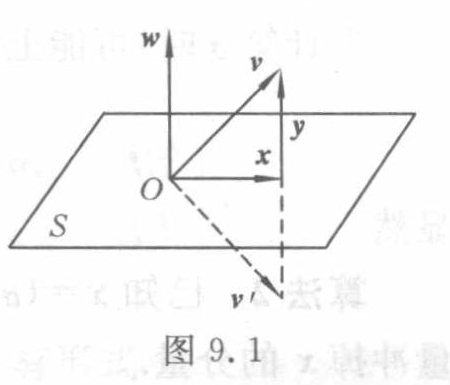
\includegraphics[width=0.85\linewidth,height=\textheight,keepaspectratio,alt={图 9.1，初等反射阵的几何意义，原图裁切}]{verified/assets/ch09a/fig-9-1.png}

图 9.1（原图裁切）。图中符号为 \(w,v,x,y,O,S,v'\)。超平面 \(S\) 经过原点 \(O\)，\(w\) 为法向量；\(v=x+y\) 分解为平面内分量 \(x\) 与垂直分量 \(y\)，\(v'\) 位于平面另一侧，表示镜面反射所得 \(x-y\)。原图用虚线连接 \(O\)、\(v'\) 端点及垂直分量方向。

初等反射阵在计算上的意义是它能用来约化矩阵，例如设向量 \(a\ne0\)，可选择一初等反射阵 \(H\) 使 \(H_a=\sigma e_1\)。这种约化矩阵的方法称为 Householder 方法。为此给出下面定理。

\textbf{定理 9.12} 设 \(x,y\) 为两个不相等的 \(n\) 维向量，\(\|x\|_2=\|y\|_2\)，则存在一个初等反射阵 \(H\)，使 \(Hx=y\)。

\textbf{证明} 令 \(w=\dfrac{x-y}{\|x-y\|_2}\)，则得到一个初等反射阵

\[
H=I-2ww^{\mathrm T}=I-2\frac{(x-y)}{\|x-y\|_2^2}(x^{\mathrm T}-y^{\mathrm T}),
\]

而且

\[
Hx=x-2\frac{x-y}{\|x-y\|_2^2}(x^{\mathrm T}-y^{\mathrm T})x=x-2\frac{(x-y)(x^{\mathrm T}x-y^{\mathrm T}x)}{\|x-y\|_2^2},
\]

因为

\[
\|x-y\|_2^2=(x-y)^{\mathrm T}(x-y)=2(x^{\mathrm T}x-y^{\mathrm T}x),
\]

所以

\[
Hx=x-(x-y)=y.
\]

易知，\(w=\dfrac{x-y}{\|x-y\|_2}\) 是使 \(Hx=y\) 成立的唯一长度等于 1 的向量（不计符号）。

\textbf{推论} 设向量 \(x\in\mathbf R^n\ (x\ne0)\)，\(\sigma=\pm\|x\|_2\)，且 \(x\ne-\sigma e_1\)，则存在一个初等反射阵

\[
H=I-2\frac{uu^{\mathrm T}}{\|u\|_2^2}\equiv I-\rho^{-1}uu^{\mathrm T},
\]

使 \(Hx=-\sigma e_1\)，其中 \(u=x+\sigma e_1\)，\(\rho=\|u\|_2^2/2\)。

设

\[
x=(\alpha_1,\alpha_2,\cdots,\alpha_n)^{\mathrm T}\ne0,\quad u=(u_1,u_2,\cdots,u_n)^{\mathrm T},
\]

\begin{quote}
\textbf{校注（agent 补充，ch09a-E008）} 在``可选择一初等反射阵 \(H\) 使''后，原图把 \(a\) 印在 \(H\) 的下标位置，故照录为 \(H_a=\sigma e_1\)。依本段语义及随后定理的矩阵作用，应为乘积 \(Ha=\sigma e_1\)；疑为原书排版错误。见\href{verified/assets/ch09a/review-p244-Ha.png}{放大原式}。
\end{quote}

\clearpage

原书 PDF 页 245；印刷页码 232。

\href{source-images/pdf-245.jpeg}{原页图像}

则

\[
u=(\alpha_1+\sigma,\alpha_2,\cdots,\alpha_n)^{\mathrm T},
\]

\[
\rho=\frac12\|u\|_2^2=\frac12\left[(\alpha_1+\sigma)^2+\alpha_2^2+\cdots+\alpha_n^2\right]=\sigma(\sigma+\alpha_1).
\]

如果 \(\sigma\) 和 \(\alpha_1\) 异号，那么计算 \(\alpha_1+\sigma\) 时有效数字可能损失，取 \(\sigma\) 和 \(\alpha_1\) 有相同的符号，即取

\[
\sigma=\operatorname{sgn}(\alpha_1)\|x\|_2.
\]

\textbf{算法 1} 已知向量 \(x=(\alpha_1,\alpha_2,\cdots,\alpha_n)^{\mathrm T}\ne0\)，本算法算出 \(\sigma,\rho\) 及 \(u\)，使 \((I-\rho^{-1}uu^{\mathrm T})x=-\sigma e_1\)，\(u\) 的分量冲掉 \(x\) 的分量。

\textbf{步 1} 计算 \(\sigma=\operatorname{sgn}(\alpha_1)\left(\displaystyle\sum_{i=1}^n\alpha_i^2\right)^{\frac12}\)。

\textbf{步 2} \(\alpha_1\to u_1=\alpha_1+\sigma\)。

\textbf{步 3} \(\rho=\sigma u_1\)。

在计算 \(\sigma\) 时，可能上溢或下溢。为了避免溢出，将 \(x\) 规范化

\[
\eta=\max_i|\alpha_i|,\quad x'=\frac{x}{\eta},
\]

显然

\[
\sigma'=\sigma/\eta,\quad H'=H.
\]

\textbf{算法 2} 已知 \(x=(\alpha_1,\alpha_2,\cdots,\alpha_n)^{\mathrm T}\ne0\)，本算法算出 \(H\) 及 \(\sigma\) 使 \(Hx=-\sigma e_1\)，\(u\) 的分量冲掉 \(x\) 的分量。

\textbf{步 1} \(\eta=\max_i|\alpha_i|\)。

\textbf{步 2} \(\alpha_i\leftarrow u_i=\dfrac{\alpha_i}{\eta}\quad(i=1,2,\cdots,n)\)。

\textbf{步 3} \(\sigma=\operatorname{sgn}(u_1)\left(\displaystyle\sum_{i=1}^nu_i^2\right)^{\frac12}\)。

\textbf{步 4} \(u_1\leftarrow u_1+\sigma\)。

\textbf{步 5} \(\rho=\sigma u_1\)。

\textbf{步 6} \(\sigma\leftarrow\eta\sigma\)。

关于 \(HA\) 的计算，设 \(A=(a_1,a_2,\cdots,a_n)\)，其中 \(a_i\) 为 \(A\) 的第 \(i\) 列向量，则

\[
HA=(Ha_1,Ha_2,\cdots,Ha_n),
\]

因此计算 \(HA\) 就是要计算

\[
Ha_i=(I-\rho^{-1}uu^{\mathrm T})a_i=a_i-(\rho^{-1}u^{\mathrm T}a_i)u\quad(i=1,2,\cdots,n).
\]

于是计算 \(Ha_i\) 只需要计算两向量的数量积和两向量的加法即可，且计算 \(HA\) 共需要 \(2n^2\) 次乘法运算。

\subsubsection{9.3.2 用正交相似变换约化矩阵}\label{ch09a-ux7528ux6b63ux4ea4ux76f8ux4f3cux53d8ux6362ux7ea6ux5316ux77e9ux9635}

下面考虑用初等反射阵来正交相似约化一般矩阵和对称矩阵。设

\clearpage

原书 PDF 页 246；印刷页码 233。

\href{source-images/pdf-246.jpeg}{原页图像}

\[
A=\left(\begin{array}{c|ccc}
a_{11}&a_{12}&\cdots&a_{1n}\\\hline
a_{21}&a_{22}&\cdots&a_{2n}\\
\vdots&\vdots&&\vdots\\
a_{n1}&a_{n2}&\cdots&a_{nn}
\end{array}\right)
\equiv\begin{pmatrix}
a_{11}&A_{12}^{(1)}\\
a_{21}^{(1)}&A_{22}^{(1)}
\end{pmatrix},
\]

\textbf{步 1} 不妨设 \(a_{21}^{(1)}\ne0\)，否则这一步不需约化，选择初等反射阵 \(R_1\) 使 \(R_1a_{21}^{(1)}=-\sigma_1e_1\)，其中

\[
\left\{
\begin{aligned}
\sigma_1&=\operatorname{sgn}(a_{21})\left(\sum_{i=2}^na_{i1}^2\right)^{\frac12},\\
u_1&=a_{21}^{(1)}+\sigma_1e_1,\\
\rho_1&=\frac12\|u_1\|_2^2=\sigma_1(\sigma_1+a_{21}),\\
R_1&=I-\rho_1^{-1}u_1u_1^{\mathrm T}.
\end{aligned}
\right.
\tag{9.3.1}
\]

令 \(U_1=\begin{pmatrix}I&0\\0&R_1\end{pmatrix}\)，则

\[
A_2=U_1A_1U_1=\begin{pmatrix}
a_{11}&A_{21}^{(1)}R_1\\
R_1a_{21}^{(1)}&R_1A_{22}^{(1)}R_1
\end{pmatrix}
\equiv\begin{pmatrix}
A_{11}^{(2)}&a_{12}^{(2)}&A_{13}^{(2)}\\
O&a_{22}^{(2)}&A_{23}^{(2)}
\end{pmatrix},
\]

其中 \(A_{11}^{(2)}\in\mathbf R^{2\times1},\quad a_{22}^{(2)}\in\mathbf R^{n-2},\quad A_{23}^{(2)}\in\mathbf R^{(n-2)\times(n-2)}\)。

\textbf{步 \(k\)} 设对 \(A\) 已进行了第 \(k-1\) 步正交相似约化，即 \(A_k\) 有形式

\[
\begin{aligned}
A_k&=U_{k-1}A_{k-1}U_{k-1}\\
&=\left(\begin{array}{ccc|c|ccc}
a_{11}&a_{12}^{(2)}&\cdots&a_{1k}^{(k)}&a_{1,k+1}^{(k)}&\cdots&a_{1n}^{(k)}\\
-\sigma_1&a_{22}^{(2)}&\cdots&a_{2k}^{(k)}&a_{2,k+1}^{(k)}&\cdots&a_{2n}^{(k)}\\
&\ddots&\ddots&\vdots&\vdots&&\vdots\\
&&-\sigma_{k-1}&a_{kk}^{(k)}&a_{k,k+1}^{(k)}&\cdots&a_{k,n}^{(k)}\\\hline
&&&a_{k+1,k}^{(k)}&a_{k+1,k+1}^{(k)}&\cdots&a_{k+1,n}^{(k)}\\
&&&\vdots&\vdots&&\vdots\\
&&&a_{nk}^{(k)}&a_{n,k+1}^{(k)}&\cdots&a_{nn}^{(k)}
\end{array}\right)\\
&\equiv\begin{pmatrix}
A_{11}^{(k)}&a_{12}^{(k)}&A_{13}^{(k)}\\
O&a_{22}^{(k)}&A_{23}^{(k)}
\end{pmatrix},
\end{aligned}
\]

其中 \(A_{11}^{(k)}\in\mathbf R^{k\times(k-1)},\quad a_{22}^{(k)}\in\mathbf R^{n-k},\quad A_{23}^{(k)}\in\mathbf R^{(n-k)\times(n-k)}\)。

设 \(a_{22}^{(k)}\ne0\)，选择初等反射阵 \(R_k\)，使 \(R_ka_{22}^{(k)}=-\sigma_ke_1\)，其中

\[
\left\{
\begin{aligned}
\sigma_k&=\operatorname{sgn}(a_{k+1,k}^{(k)})\left(\sum_{i=k+1}^na_{ik}^2\right)^{\frac12},\\
u_k&=a_{22}^{(k)}+\sigma_ke_1,\\
\rho_k&=\frac12\|u_k\|_2^2=\sigma_k(\sigma_k+a_{k+1,n}^{(k)}),\\
R_k&=I-\rho_k^{-1}u_ku_k^{\mathrm T}.
\end{aligned}
\right.
\tag{9.3.2}
\]

\begin{quote}
\textbf{校注（agent 补充，ch09a-E009）} 本页 \(A_2\) 的二阶分块表达式右上块原印 \(A_{21}^{(1)}R_1\)，已照录。由页首定义的右上块 \(A_{12}^{(1)}\) 和 \(U_1\) 的分块乘法，此处应为 \(A_{12}^{(1)}R_1\)。见\href{verified/assets/ch09a/review-p246-initial-partition.png}{页首分块}和\href{verified/assets/ch09a/review-p246-A-2.png}{放大原式}。

\textbf{校注（agent 补充，ch09a-E010）} 式（9.3.2）原图 \(\sigma_k\) 求和内为 \(a_{ik}^2\)，未印迭代上标；\(\rho_k\) 最后一个矩阵元为 \(a_{k+1,n}^{(k)}\)，均照录。由本页 \(a_{22}^{(k)}=(a_{k+1,k}^{(k)},\ldots,a_{nk}^{(k)})^{\mathrm T}\) 和 \(u_k=a_{22}^{(k)}+\sigma_ke_1\)，求和应使用当前列元素 \((a_{ik}^{(k)})^2\)，而范数平方恒等式给出 \(\rho_k=\sigma_k(\sigma_k+a_{k+1,k}^{(k)})\)。故前者疑漏迭代上标，后者列下标疑将 \(k\) 印成 \(n\)。见\href{verified/assets/ch09a/review-p246-9-3-2.png}{放大原式}。
\end{quote}

